\documentclass{article}
\usepackage[utf8x]{inputenc}
\usepackage{default}
\usepackage{graphicx}
\usepackage{amsmath}
\usepackage{hyperref}
\usepackage[sort&compress]{natbib}
\usepackage[a4paper,total={6in,9in}]{geometry}

\def\wp{\omega^\prime}
\def\w{\omega}
\def\wc{{\omega_{\rm C}}}
\def\ket{\rangle}
\def\bra{\langle}
\def\H{\hat{H}}
\def\P{\hat{P}_{\rm occ}}
\def\E{\varepsilon}
\def\vp{{v^\prime}}
\def\q{{\bf q}}
\def\s{\sigma}
\def\k{{\bf k}}
\def\qp{{\bf q^\prime}}
\def\G{{\bf G}}
\def\Gp{{\bf G^\prime}}
\def\rt{\tilde{r}}
\def\pt{\tilde{p}}
\def\r{{\bf r}}
\def\R{{\bf R}}
\def\rp{{\bf r^\prime}}
\def\rpp{{\bf r^{\prime\prime}}}
\def\rppp{{\bf r^{\prime\prime\prime}}}
\def\x{{\bf x}}
\def\mo{$\overline{1}$}
\def\mt{$\overline{2}$}
\def\S{\mathcal{S}}
\def\Gs{\mathcal{G}}
\def\v{\mathbf{v}}
\def\symm{\left\{\mathcal{S}|\mathbf{v}\right\}}
\def\g{\mathcal{g}}

\usepackage{soul}
\usepackage{color}
\usepackage{subfig}

\definecolor{yellow}{rgb}{1,1,0}
\definecolor{lightblue}{rgb}{0.6,0.6,0.9}
\sethlcolor{yellow}

\begin{document}
\title{The GW approximation and Tight Binding Recursion}
\author{Henry Lambert}
\date{\today}
\maketitle

\section{Introduction}
  Vol. 35 of Solid State Physics is dedicated to electronic structure
physics from the point of view of the local environment. This perspective
has a long tradition in physical and chemical electronic structure theory.
The theory has a certain intuitive appeal and follows naturally from 
the early progress in quantum mechanics. 

Initially understanding of quantum mechanics came from the study
of black body radiation, the hydrogen atom, photoemission phenomenon, 
and electron diffraction experiments. From 
the understanding of the electronic states of hydrogen emerged the
understanding of larger atomic systems. Hartree theory and Hartree-Fock
theory, the latter of which includes the exchange interaction arising 
from Pauli's work on the statistics of fundamental particles 
provided access to the wave functions of these many electron 
atomic systems. Similarly the susceptibility of atomic
systems was investigated at an early stage via perturbation theory.
As the mechanics of atoms came t  be understood it was natural 
to base subsequent theories of the mechanics
of electrons in crystals and solids as an extension of atomic theory.

From this shared intellectual heritage emerged the many tribes of present
day electronic structure theory. The tribes are well known 
to practicioners in the field, approaches, some of which we could name 
here, Linear combination of atomic orbitals(LCAO), 
linear muffing tin orbitals (LMTO), plane waves
and pseudopotentials, gaussian orbitals, tight binding formalisms, 
Kohn-Kuttinger-Rostiger theory.

\section{The Invariance Theorem}
\label{sec:invariance}
Heine presents an extended discussion of the invariance
theorem. Heine's section begins, by way of introduction, by pointing 
out an analogy between  the the local density of states of a system of interacting
electrons and the black body spectrum of electromagnetic radiation.

The analogy can be seen by writing the density of states,
and the local density of states (for each spin direction) as:

\begin{eqnarray}
n(E) = \sum_{n}\delta(E-E_{n}) \\
n(E,\r) = \sum_{n} |\psi_{n}(\r)|^{2}\delta(E-E_{n})
\end{eqnarray}

and the density of black-body radiation $\rho(\omega,\r)$
with the substitution of the wavefunction with the electromagnetic
field and the energy level with a frequency $\omega$.

The local density of states is related in turn to the 
Green's function of a system:
\begin{equation}
n(E,\r) = -\frac{1}{\pi}{\rm Im} G(\r,\r',E)
\end{equation}

These tools should be more than sufficient to investigate what
we are interested in: namely cohesive properties, magnetic moments
and localized atomic forces in clusters. The math
should also be sufficient to devising schemes that allow for the correction
of artificial effects introduced into numerical work from the appearance
of spurious surfaces.

Heine's ambition turns on this:
\begin{quote}
We see now that the trick in the new formulation of quantum 
mechanics is not just to express measurable quantities in terms of 
G, {\emph but in terms of some appropriate small parts of G that can be solved 
for and computed separately from all the unwanted remainder of G.}
\end{quote}

This relies, again in analogy with black bodies, on the Green
function being independent of the size and shape
of the container (of electrons) and the boundary conditions.


First a change of variables is perform from r to r'' in 4.1 and r to r'' and r'
to r in 4.3
\begin{equation}
\label{eq:greentot}
[-\frac{1}{2}\nabla^{2}_{\r''} + V(\r'') - E]G(\r'',\r',E)= -\delta(\r''-\r')
\end{equation}

\begin{equation}
\label{eq:greenA}
[-\frac{1}{2}\nabla^{2}_{\r''} + V(\r'') - E]G_{A}(\r,\r'',E)= -\delta(\r''-\r')
\end{equation}

Now multiply Eq. \ref{eq:greentot} by $G_{A}$ and Eq.
\ref{eq:greenA} by $G$ Then integrate over r'' over region A using
Green's theorem:

\begin{equation}
\label{eq:greenthm}
\int\int\int(\phi\nabla^{2}\psi - \psi\nabla^{2}\phi)d^{3}\r 
= \int(\phi\nabla\psi-psi\nabla\phi)d{\mathbf{S}}
\end{equation}
 One then obtains

Subsuming the energy arguments we obtain an
expressions for G by integrating r'' over region A.

\begin{equation}
\label{eq:green1a}
G(\r,\r') = G_{A}(\r,\r') + \frac{1}{2} \int d\mathbf{S} 
[\frac{\partial G_{A}(\r,\r_{s})}{\partial n_{S}}G(\r_{S},\r')
- G_{A}(\r,\r_{S})\frac{\partial G(\r_{S},\r')}{\partial n_{S}} [\r, \r' \in A]]
\end{equation}

$\frac{\partial}{\partial n_{S}}$ denotes the normal component of grad across
the surface S and $\r_{S}$ is a point on S. (The grad term is a directional component
so can induce a change in sign!)

And in region B:
%
\begin{equation}
\label{eq:green1b}
G(\r,\r') = G_{B}(\r,\r') - \frac{1}{2} \int d\mathbf{S} 
[\frac{\partial G_{B}(\r,\r_{s})}{\partial n_{S}}G(\r_{S},\r')
- G_{B}(\r,\r_{S})\frac{\partial G(\r_{S},\r')}{\partial n_{S}} [\r, \r' \in B]]
\end{equation}
%

A further property has been used:
%
\begin{equation}
G(\r,\r',E) = G(\r',\r,E)
\end{equation}
%
which is often justified on the ground of a time reversal theorem
applying to the wave functions.

Finally consideration of r' and r'' in different regions is required.

With $\r''$ in B and $\r'$ in A Eq.~\ref{eq:greentot} becomes:
%
\begin{equation}
[-\frac{1}{2}\nabla^{2}_{\r''} + V(\r'') - E]G(\r'',\r')=0,
\end{equation}
%
the delta function is uniformally zero with those spatial constraints.

The next case restricts $\r$ in B:
%
\begin{equation}
[-\frac{1}{2}\nabla^{2}_{\r''} + V(\r'') - E]G_B(\r,\r'')= \delta(\r-\r''),
\end{equation}
%

A similar cross multiplying trick gives:
%
\begin{equation}
\label{eq:green1c}
G(\r,\r') = -\frac{1}{2} \int dS[\frac{\partial G_{B}(\r, \r_{S}}{\partial n_{S}} G(\r_{S},\r')
- G_{B}(\r, \r_{S})\frac{\partial G(\r_{S},\r'}{\partial n_{S}}] [\r in B, \r' in A],
\end{equation}
%
and a similar relation for [$\r$ in A and $\r'$ in B].

Eq.~\ref{green1a} and Eq.~\ref{green1b} give solutions for G but 
aren't very useful until the terms
$G(\r_S,\r)$ and $\frac{\partial G}{\partial n_{S}}$ are eliminated.

From Eq.~\ref{eq:green1a} we let $\r$ tend to the boundary so $\r = \r_{S}$
%
\begin{equation}
\label{eq:greensys1}
G(\r'',\r') = G_{A}(\r''_{S}, \r') + \frac{1}{2} \int d{S}
[\frac{\partial G_{A}(\r''_{S}, \r_{S})}{\partial n_{S}} G(\r_{S},\r) - 
G_{A}(\r''_{S},\r_{S})\frac{\partial{G(\r_{S}, \r')}{\partial n_{S}}}].
\end{equation}
%

The second relation comes from Eq.\ref{eq:green1c} with 
$\r$ in region B and letting $\r$ tend to $\r^{''}_{S}$.
%
\begin{equation}
\label{eq:greensys2}
G(r''_{S}, \r') = -\frac{1}{2}\int dS [\frac{\partial G_{B}(\r''_{S}, \r_{S})}{\partial n_{S}}
-G_{B}(\r''_{S},\r_{S})\frac{\partial G(\r_{S},\r')}{\partial n_{S}}]
\end{equation}
%

We now dump the cumbersome indices on the position attributes. These
were necessary to motivate the physical argument for how we have a Green's function
description in one region of space, a Green's function description in another, 
and the joined physical system should be some combination of these two descriptions
which match at the interface. The final step is to write Eq.~\ref{eq:greensys1} 
and Eq.~\ref{eq:greensys2}.


\begin{eqnarray}
\label{eq:operator1}
\g = \g_{A} + \frac{1}{2}\G'_{A}\g - \frac{1}{2}\G_{A}\g' \\
\g = -\frac{1}{2}\G'_{B}\g + \frac{1}{2}\G_{B}\g' \\
\end{eqnarray}

\begin{eqnarray}
\label{eq:operator2}
\g = [\G^{-1}_{A}(1-\frac{1}{2}\G'_{A}) + \G^{-1}_{B}(1+\frac{1}{2}\G'_{B})]^{-1} \G^{-1}_{A}\g_{A}
\g'= [(1-\frac{1}{2}\G'_{A})^{-1}\G_{A} + (1+\frac{1}{2}\G'_{B})^{-1}]^{-1}(1 - \frac{1}{2}\G'_{A})^{-1}2\g_{A}
\end{eqnarray}

$\g$, $\g_{A}$, $\g'$ are vectors in a space $\{\r_{S}\}$ with components $G(\r_{S},\r')$,
$G_{A}(\r_{S},\r')$, $\partial G(\r_{S},\r')/\partial n_{S}$ with $\r'$ fixed and
$\G_{A}$, $\G'_{A}$ are operators in the space with matrix elements
$G_(A)(\r''_{S}, \r_{S})$, $\partial G_{A}(\r''_{S}, \r_{S})/\partial n_{S}$.

Where the inverse in Eq.~\ref{eq:operator1, eq:operator2} 
doesn't exist there is a pole and this is the condition
for a discrete energy level of the Schrodinger equation 
for the combined A + B systems. 

Equations written in the form of \ref{eq:green1a} are of the type required for the invariance theorem namely:
\begin{equation}
G(\r,\r') = G_{A}(\r,\r') + {\rm boundary corrections}.
\end{equation}

These considerations provide a reasonable mathematical framework for 
investigating electronic structure from the point of view of the local environment.

\section{Recursion Method}
The principle of the recursion method, the details of the calculation will follow, is 
to obtain an efficient expression for a diagonal element of the Green's function.

\begin{equation}
G_{\chi\chi}(E) = \bra\chi|[E + i\delta -H]^{-1}|\chi\ket
\end{equation}

\begin{equation}
n_{\alpha l}(E) = -\frac{1}{\pi} {\rm Im}\bra\alpha l|[E + i\delta -H]^{-1}|\alpha l\ket
\end{equation}

$\chi$ can be made up of some linear combination of the local basis set $\phi_{\alpha l}$,
which, in turn, could be local atom centered orbitals, of bond orbitals, 
or even atomic diplacements to describe lattice vibrations. The method is thus
applicable to a wide range of problems in condensed matter.

\begin{equation}
b_{n+1}|u_{n+1}\ket = H |u_{n}\ket - a_{n}|u_{n}\ket - b_{n}|u_{n-1}\ket
\end{equation}

\subsection{Mathematical Origin}
The trick of the recursion method, if you like to think of things in terms of tricks, 
or its generating feature, if you prefer, is that from the outset the `greenian' is constricted
to the particular starting orbital $u_{0}$: 
%
\begin{equation}
G_{\alpha l, \alpha l}(E) = \bra u_{0}|[E-H]^{-1}|u_{0}\ket 
\end{equation}
%
As Heine puts it in his chapter:
%
\begin{quote}
Note that we do not want the whole of the inverse matrix $[E-H]^{-1}$, 
\emph{only one element}. and on this the whole method depends. In physics we do not
usually inquire about the whole of life, but about one particular matrix element (at a time) and we have chosen
$u_{0}$ so that \ref{eq:greenian} gives us what, to put it crudely, we want.
\end{quote}

%
\begin{equation}
\bra u_{0}|[E-H]^{-1}|u_{0}\ket = \frac{{\rm det}|D_{1}|}{{\rm det}|D_{0}|}
\end{equation}
%

This can be equivalently written as:
\begin{equation}
\bra u_{0}|[E-H]^{-1}|u_{0}\ket = \frac{1}{\frac{{\rm det}|D_{0}|}{{\rm det}|D_{1}|}}
\end{equation}

Appeal is then made to Cauchy for the following expansion:

\begin{equation}
{\rm det}|D_{0}| = (E-a_{0}){\rm det}|D_{1}| - b^{2}_{1}{\rm det}|D_{2}|
\end{equation}

and when generalized to determinants for $|D_{n}|$, $|D_{n+1}|$, and $|D_{n+2}|$:

\begin{equation}
\frac{{\rm det}|D_{n}|}{{\rm det} D_{n+1}} = E-a_{n}) - \frac{b^{2}_{n+1}}{\frac{{\rm det}|D_{n+1}}{{\rm det}|D_n+2|}}
\end{equation}

\subsection{Integrated Quantities and Energy Difference between Two Substructures}
Some integrated quantities over the density of states of interest would be
the electron occupancy of a specific orbital:
%
\begin{equation}
N_{\alpha l}(E) = \int_{-\infty}^{E_{F}}E' n_{\alpha l}(E') dE'
\end{equation}

The total energy in a particular orbital is also convergent with increasing cluster size:
%
\begin{equation}
U_{d} = \int_{-\infty}^{E_{F}}E'n_{\alpha l}(E') dE'
\end{equation}
%

Lets calculate energy difference of two structures A and B for the same transition metal
in fcc and hcp structures.
%
\begin{eqnarray}
\label{eq:Ua}
U_{A} = \int_{-\infty}^{E_{FA}} E n_{A}(E) dE
\end{eqnarray}

\begin{eqnarray}
\label{eq:Ub}
U_{B} = \int_{-\infty}^{E_{FB}} E n_{B}(E) dE
\end{eqnarray}

\begin{equation}
\label{eq:totaldos}
Z = \int_{-\infty}^{E_{FA}} n_{A}(E)dE = \int_{-\infty}^{E_{FB}}n_{B}(E)dE
\end{equation}

\begin{equation}
U_{A}-ZE_{FA}= \int_{-\infty}^{E_{FA}}(E-E_{FA})n_{A}(E)dE
\end{equation}

\begin{equation}
U_{B}-ZE_{FA}= \int_{-\infty}^{E_{FA}}(E-E_{FA})n_{B}(E)dE + \int_{E_{FB}}^{E_{FA}}n_{B}(E)dE
\end{equation}

If $n_{B}(E)$ is taken to be constant across that small energy range, the second term, in
Eq. results in a small squared term that can be dropped. Swapping $E_{FB}$ and $E_{FA}$ gives
a similar result. This justifies dropping the A index on the Fermi energy to get the
final expression:
%
\begin{equation}
U_{A}-U_{B} = \int_{-\infty}^{E_{F}}(E-E_{F})[n_{A}(E) -n_{B}(E)]dE.
\end{equation}
%
It is this expression used to separate the Lave phases of transition metals in  Ref.~\cite{haydock76}.

\section{Kelly}
An example from Kelly helps to make the shape of the Hamiltonian absolutely 
concrete.

\begin{quote}
As input data we require a convenient local representation of H. In simple crystals,
this is most easily given in terms of interactions with a unit cell and between neighboring cells.
For a fcc transition metal we have nine orbital (1s, 3p, 5d) per site, and a diagonal 9x9 matrix
for the self-energies of these orbitals. Twelve 9x9 matrices suffice to describe the interaction 
of any atom with its neighbors.
\end{quote}

And it is probably worth noting at this stage, for the practically minded,  
that the actual operations of $H|u_{n}\ket$ can be written as:
%
\begin{equation}
H|u_{n}\ket = \sum_{\alpha l \beta j}a_{n \alpha l}(\bra \beta j |H| \alpha l\ket)|\beta j\ket,
\end{equation}
%
and since we wish to exploit the sparsity of H we introduce an index $z$ which
runs over the neighbors of site l with which the orbitals interact:
\begin{equation}
H|u_{n}\ket = \sum_{\alpha l z}a_{n \alpha l}(\bra \beta_{z} j_{z} |H^{z}|\alpha l\ket)|\beta_{z} j_{z}\ket.
\end{equation}

There are no restrictions on the number of orbitals per site, or on the range of interactions that can be
incorporated, these only impact on the efficiency of the method and the validity of the original assumptions
about the dominance of the local atomic environment.

\section{Aside Green's Function Matching}
I would argue that every plane wave/pseudopotential calculation is in fact
an example of Green's function matching. Between atoms a basis of plane
waves describes interatomic bonding. In the vicinity of ions a pseudopotential
describes the way these plane waves are scattered at the atomic sites.
Indeed the logarithmic derivatives are required to match 
that of the atomic wavefunction at the cutoff radius for the pseudopotential.

\section{Free Electrons}
\begin{equation}
H = - \hbar^{2}/2m \nabla^{2}
\end{equation}

In spherical co-ordinates:
%
\begin{equation}
H = \frac{hbar^{2}}{2m}(d/dr^{2}  ) 
\end{equation}

\section{Future Work}
The chain model has been used in numerical work as a way of 
diagonalizing matrices in a computer 
C. Lanczos J. Res. Natl. Bur. Stand. 45, 255 (1950) and
by Chebyshev for approximating functions on an interval
P. L. Chebyshev, Bull. Acad. Imp. Sci. St. Petersbourg 1, 193 (1859)

What we wish to examine, is determined by $u_{0}$, this could be a combination
of neighbouring orbitals if we wish to determine the bond order, if it is the electronic
structure at a surface, the $u_{0}$ should be a state at the surface, and similarly if it
is a bulk state we wish to probe.

The references in Vol. 35 demonstrate the scope of application of the method 
already achieved by 1980. A subset of those works have been referenced here. 
Haydock's conclusion is interesting in he gives prognosis for further work
along two lines: the extension to many-body Hamiltonians.

\begin{quote}
One of the outstanding problems is that of the Anderson model
of a disordered solid. Here the Hamiltonian is defined statistically and
one would like to transform to a corresponding statistically defined chain where
one could discuss the distributions of various physical quantities.
\end{quote}

\begin{quote}
  Finally, the reader may have noticed that the approach of this chapter has been entirely directed
toward independent particle models. However, many-body Hamiltonians must be similarly 
transformable to chain models. Aside from a small amount of thought and continuing interest, 
nothing has been done about this and it remains a most interesting problem concerning recursive 
solution of the Schrodinger equation.
\end{quote}

\section{Intermediate Epilogue}
Work did continue in this field and \cite{annett94}. There the LDOS is extended
to the PDOT projected density of transitions and it is argued singularities
in the PDOT correspond to thresholds for creating long lived elementary excitations 
of the many body system.

\section{Many Body Recursion}


\label{sec:manybodyrecursion}
	Since Vol. 35 was published there has been a rise in the accessibility of density functional methods 
and the access to good single particle approximations to the electronic eigenstates of a crystal
is routine. Additionally progress on the problem of determining unique approximations to localized
electronic states, Wannier functions, means tight binding Hamiltonians can be parameterized directly
rather than via fits to band structures and relying on physical intuition. Finally ab initio many body
calculations have also proved quite successful

A many body Hamiltonian amenable to being written in a sparse format might look like this:
%
\begin{equation}
H = [\frac{1}{2}\nabla^{2} + \tilde{v}_{\rm loc} + \hat{\Sigma}(\r,\r';\omega)]
\end{equation}
%
	$\Sigma(\r,\r';\omega)$ is a self energy operator, it is not local and 
has an additional argument that includes the energy.
If we impose a requirement that spatial integrals over $\Sigma$ can be performed in 
well defined atom centered regions of space. For instance 
the first neighbour interaction is now formally written as: 
%
\begin{equation}
\int_{\Omega_{j}}<w_{i}(r-R)|\sigma(\R,\r';\omega)|w_{j}(r-R)>d\r'
\end{equation}
%
	Subsequent neighbour interactions would take a similar form
with the integration region, $\Omega_{j}$ being a Wigner cell around an 
atom j. In order for the scheme to be sensible the contributions from subsequent shells 
must be negligible. This is likely to be the case so long as $w$ and/or $\Sigma$ 
are falling off quickly enough. Which, as will become clear when we discuss
the relationship of this scheme to the GW approximation, requires 
the Green's function or the screened Coulomb interaction 
to be sufficiently localized.

The on-site self-interaction term can be computed as
%
\begin{equation}
\int_{\Omega_{i}}<w_{i}(r-R_{i})|\sigma(\r,\r';\omega)|w_{i}(r-R_{i})>d\r'd\r
\end{equation}
%
If $\Sigma$ is chosen to be Hermitian a self-consistent calculation 
becomes tractable resulting in a new collection of single particle 
states with higher order polarization and exchange terms included 
in their summation the SC-GW is an example of this procedure. The more of
these processes that can be included in the single particle configuration of the
system the better the tight binding guess is likely to be. The self-consistency
in the recursion method relies on the adjustment of the $\Sigma$ operator and the
fewer depths of recursion required to stabilize this quantity the more efficient the
scheme can be considered.

In principle we can now compute any quantity we like that can be expressed
as a density of states, or an integral over the density of states.
The basis set may remain an issue. The localized functions will not have the 
flexibility of planes waves so if we seek the green's function in the 
region of the plasmon energies our basis set might not have the flexibility 
to describe that solution? I'll have to think about this. Ultimately the 
solution for the resolvent at those energies i.e. $ImG_{nk}(\omega)$ should 
reproduce what I'm looking for. The test for this would be with Si, if 
I can reproduce spectral functions with TB recursion that is a legitimate 
proof of concept and would clarify the extent to which collective excitations,
plasmon, can be incorporated in TB recursion. The difficulty of 
Van Hove singularities suggests we might be at cross purposes...

Also Writing the equations in this way and the proposed method of solution
yield some post hoc justification for parameterizations of plasmon
pole models or the use of Pad\'e approximants to capture the frequency dependence
of the key operators.

Similarly the contributions of neighbours to the self-energy 
operator yields some physical insight.

A good first order approximation to $\Sigma$ comes from the GW approximation.
We will write matrix elements of this to see the connection between the
recursion method and the calculation of $\Sigma$. 
%
\begin{equation}
\label{eq:sigma}
\Sigma_{ij}(\omega) = <\phi_{i}|\int G(\omega-\omega')W(\omega')d\omega'|\phi_{j}>
\end{equation}
%
	We now insert the identity operator into Eq.$\sigma$ strategically and at 
a number of places:
%
\begin{equation}
\label{eq:sigma}
\Sigma_{ij}(\omega) = <\phi_{i}|\int G(\omega')\sum_{n}|\phi_{n}><\phi_{n}|(G(\omega')|\phi_{n}><\phi_{n}|G(-\omega')v)d\omega'|\phi_{j}>
\end{equation}
%
\begin{equation}
\label{eq:sigma_onsite}%need to check the frequency polarization expression
\Sigma_{ii}(\omega) = <\phi_{i}|\int G(\omega')\sum_{n}|\phi_{n}><\phi_{n}|(G(\omega')|\phi_{n}><\phi_{n}|G(-\omega')v)d\omega'|\phi_{i}>
\end{equation}
%
	The insertion of multiple identity operators
makes our scheme clear: the mechanics of the recursion method 
can now be fully exploited. All that is required to compute the self energy 
operator is a number of Greenian's for $G_{ij}(\omega)$ which we will
initialize however we like. These will modify the coefficients at the
off diagonal elements and on the onsite terms. The closed form
expressions for $G_{ij}(\omega)$ means we have a rigorous 
energetic description $\omega$ and the values of the greenian 
can be tabulated and then reused in the solution of \ref{eq:green}.
We can now make a variety of choices to compute the on site self interaction
i.e. where G only couples on site terms, in the fashion of a hubbard U model,
and a variety of approximations i.e. is the screening local or extended.
For this scheme to be workable we again stress that the system interaction
must be sufficiently local such that $Sigma_{ij}$ matrix elements can be
calculated.

Alternatively the PDOT method might be more appropriate for calculating W.

\begin{figure}
\includegraphics{schematicpolestructure.pdf}
\end{figure}

I think Umari's operator for $|\phi><\phi|$ would be the best one!
We then have the continuum states as $e^{i\G\cdot\r}-<G|w_{i}(r-R)>$,
with occupied and low lying conduction manifold represented as Wannier 
functions.

	Although this is essentially just a rewriting of Hedin's equations
it has practical consequences. The present method eliminates
burdensome storage of what are in practice gigantic Green's function, 
screened coulomb and self energy matrices. It also eliminates the need for 
numerical integrations and convolutions. These savings are
obtained at the price of a nested call stack of recursions which 
in principle must be infinite. This may seem troubling but we do intend to truncate
the level of recursion at some point 

	Careful, justified, selection of the initial wave functions and tight binding parameters
is also required and these quantities (if they are not chosen to be analytic and approximate)
must be computed and stored. However work done on Wannier functions makes this a very
practical route. We will now embark on some numerical work in the hope that satisfactory 
results can be obtained by truncation of the terms. In particular the dielectric constant
and the plasmon frequency should emerge from this representation. These quantities
might be considered $\rho_{1}$ off diagonal long range order i.e. macroscopic parameters
that arise from the microscopic phase locking of electronic states in a crystal. See
\ref{sec:odlro} for a further discussion of this.


\subsection{Application of Recursion Method to the Electron Gas}
	We now wish to apply the ideas discussed in section \. Specifically to 
calculate the exchange-correlation energy of an electron gas. Again it is 
no coincidence that the Pad\'e approximant is used. The coefficients
of a Pad\'e approximant can be calculated via a recursive algorithm
as a continued fraction \cite{vidbergserene} and, from the physical
intuition of the local environment, this is the appropriate functional form.

The idea would be to initialize spherically localized electrons in a box 
(where the box size determines the effective electron density)
then let them diffuse and calculate the contribution to the
single particle energy and the exchange correlation energy. 
If there is a clever choice of grids and co-ordinate systems this
should be easier to compute.

This is in line with the original work of Ceperley and Alder \cite{ceperley80} except 
instead of a diffusive Monte-Carlo approach we exploit the
recursion method to obtain analytic approximations to the energy.
In their case the trial function is a product
of two-body correlation factors times a Slater determinant of 
single-particle orbitals. The two-body correlation factors are
chosen such that they remove exactly the singularities in the local energy when two electrons
approach each other. The single particle states are plane waves
in the fluid phase: when the system is polarized, to allow for there only being
one spin per spatial state, the fermi wave vector is increased to allow
for twice as many spatial orbitals. 

In the crystal phase the orbital are Gaussians centered 
at body-centered cubic lattice sites. Their simulations were typically 
for 38-248 electrons.

At each density the energy was extrapolated to an infinite number of particles
%
\begin{equation}
E(N) = E_{0} + E_{1}/N + E_{2}\Delta_{N}
\end{equation}

$E_{1}$ arises from the potential energy due to the correlation between a particle and its images
$E_{2}$ comes from the discrete nature of the Fermi sea for finite systems, $\Delta_{N}$ is the 
size dependence of an ideal Fermi system.

More details on the technique are given in an earlier version of the paper
\cite{ceperley78}. The BDJ wavefunction is written

\begin{equation}
\psi_{T}(R) = D(R) {\rm exp}(-\sum_{i<j} u(|\r_{i}-\r_{j}|))
\end{equation}
%
where D(R) is a Slater determinant of plane waves, separate slater determinants for
spin-up and spin-down particles in the unpolarized phase. The $u(r)$ is a pseudopotential
with a repulsive character and is intended to account for the particle correlation. 
(We will come back to this).

The issues of Van Hove singularities will be apparent in a recursion treatment because 
the formal solution to electron gas problems involve the creation of plasma modes.


\subsection{Application to Long Range off Diagonal Order}
The advantage of tight binding is it allows us to think in a co-ordinate space representation
of electronic structure and still obtain accurate results mainly by exploiting our notions
of locality and appealing broadly to the invariance theorem discussed by Heine and introduced
in the first part of this note. Yang presents the local diagonal order present in crystalline materials
and represent $\rho_{1}$ (the single particle density matrix) results in the 
creation of a macroscopic variable the strain, but does not precise what the macroscopic 
analog is for off diagonal long range order. Progessively higher density matrices are 
written with index n. Yang's insight is condensed in the following quotation.
%
\begin{quote}
It thus seems that in a macroscopic system, ODLRO can set in 
at $\rho_{n}$. The theorems of II indicate that
the reduced density matrix, to be called $\rho_{m}$, of lowest
order which has ODLRO must operate on a basic group that consists 
of an even number of fermions and any number of bosons. For liquid He II the basic
group is the He atom; for superconductors the basic group is a set of two electrons.
For $\rho_{m}$ the largest eigenvalue is of the order of N. It has an ODLRO
in the sense that in coordinate representation, when the unprimed coordinates are
microscopically close to a point $\x$, and the primed coordinates are microscopically
close to another point $\x'$. with $\x$ and $\x'$ macroscopically apart, $rho_{m}$
remains nonvanishing. For fixed unprimed coordinates microscopically
close together, the region of the primed coordinates where
$\rho_{m}$ remains nonvanishing is thus a "tube" with one 3-space dimension 
extending macroscopically. The volume of the region is 
\end{quote}
\begin{equation}
\Omega \times ({\rm microscopic\ dimension})^{m-1}
\end{equation}
%

The analogy between Bloch's solution for wavefunctions in a crystal is also worth
repeating in its entirety.

\begin{quote}
  The difference in the behavior of $R$ under changes in $\Phi$ for the cases 
with and without ODLRO is quite similar to the Bloch eigenvalue problem
in a periodic potential. Bloch showed that wave functions should be sought 
that changes by a phase factor $e^{i\Phi}$ for each lattice displacement. How does the 
wave function depend on $\Phi$? If the wave function remains finite between lattice points, 
the energy value and the wave function would be dependent on $\Phi$. If, however, 
the wave function becomes very small in a region between lattice points, 
caused by, e.g., a potential barrier, then the energy and the wave function 
would not be very much dependent on $\Phi$. For an infinite potential barrier in 
between the atoms, the wave function vanishes in the barrier, and the energy 
levels would be independent of $\Phi$ while the
wave function only picks up phase factors $e^{i\Phi}$ from one atom to the next.

  The physical meaning of the effect of the presence of ODLRO on the 
phase condition (36) is the, ODLRO preserves the memory of phases over 
macroscopic distances. Also in this sense, one can interpret for the 
Bloch problem, the effect of the small nonvanishing interatomic 
value of the wave function on the C dependence of the energy: 
The nonvanishing interatomic value of the wave function preserves the 
memory of phases from one atom to the next.

\end{quote}

This paper gives the first description of Bloch's function I have really understood. 
It also provides a sound mathematical basis for the pairing mechanism in BCS
superconductivity in the proof of Theorem 6 which Yang gives in the appendix.
The R spacing argument can be applied to the electrons. The strip equivalent
is microscopic (around the atom) but the spacing between phase locked electrons
is of the order of the lattice constant.

Moreover, Yang's formalism suggests that the formation of the superconducting state
can be understood in the same mathematical terms as the formation of the solid state.
The formation of a superconducting current should be no more surprising than the formation
of extended crystals.


\section{Bullet Tight Binding d-electrons.}
Bullet discusses some of the problems with treating d electrons in a tight binding 
formalism (Sec. IV 13 Solid State Physics Vol. 35). Fig. \ref{fig:datoms} demonstrates
one of the main issues arising with d electrons:
\begin{figure}
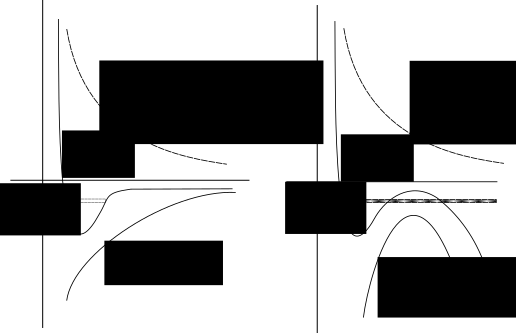
\includegraphics{resonant-datoms.pdf}
\caption{The possibility of free electron states resonating with localized states.
The centrifugal components of the atomic d wave scattering channel can combine with
the atomic potential to produce a bound electronic state at some energy $E^{0}_{l}$ for an atomic system.
In a crystal the atomic potential is periodic and in the interstitial regions electrons in an 
atomic d-like state can tunnel through the barrier localizing them and mix with free electron 
plane wave states. This dual character of localized components and extended components requires careful 
detangling to return to a tight binding description without any energy dependence 
of the matrix elements. See the discussion in the text and the work
of Pettifor in the references.}
\end{figure}

From pseudopotentials we are familiar with having to match the logarithmic energy
derivative at some cutoff radius. Usually found by integrating the radial
Schr\"odinger equation to find $u_{l}(\r,\epsilon)$ and matching the logarithmic derivatives:
%
\begin{equation}
L_{l}(\epsilon) \equiv \frac{u'_{l}(\r_{0},\epsilon)}{u_{l}(r_{0},\epsilon)} = \frac{\kappa[j'_{l}
(\kappa r_{0}) - tan \eta_{l} n'_{l}(\kappa r_{0})]} {j_{l}(\kappa r_{0}) - tan \eta_{l} n_{l}'(\kappa r_{0})]},
\end{equation}
%
where
\begin{equation}
\label{eq:phaseshift}
\tan \eta_{l} = \frac{\kappa j'_{l} - L_{l}j_{l}}{\kappa n'_{l} - L_{l}n_{l}}.
\end{equation}

In terms of the energy and width the l=2 phase shift Eq. \ref{eq:phaseshift} 
can be written:
%
\begin{equation}
\label{eq:dshift}
\tan \eta_{d} = \frac{\frac{1}{2}W(\epsilon)}{\epsilon_{d}-\epsilon}.
\end{equation}
%

The strong centrifugal contribution to the
atomic scattering potential from higher angular moment channels means the effective potential
can create a bound atomic state. In a solid the energy of this bound state can match the 
energy of a free electron state in the interstitial region and there will
be resonant tunneling between the two states. This results in the hybridization of d states
and plane waves. 

This means an appropriate model Hamiltonian must account for the various states as

\begin{eqnarray}
\label{eq:d-hamiltonian}
H = d-d  & d-PW \\
    PW-D & PW-PW \\
\end{eqnarray}
where d-d and PW-PW are of the tight-binding and plane-wave 
pseudopotential form and hybridization occurring in the 
off diagonal elements. 

These difficulty have been addressed in a number of works 
see, for example, D.G. Pettifor, J. Phys. C 5 97 (1972).
J. Hubbard Proc. Phys. Soc. London 92 921 (1967),
J. Hubbard and N. D. Dalton, J. Phys. C 1 1637 (1968),
and J. Jubbard, ibid 2, 1222 (1969). The problem being to define an
energy independent Hamiltonian, amenable to tight binding for the d electrons.

The $dd\sigma$ terms behave roughly as \cite{pettifor71}:
%
\begin{equation}
\label{eq:pettifor}
dd\sigma \approx \frac{-5W\cos\kappa_{d}R}{\kappa_{d}R}
\end{equation}
%
If we write our basis functions in terms of localized orbits this long range hopping of
Eq.~\ref{eq:pettifor} is  precisely Yangs long range off diagonal order, in fact if 
the energy is equal to $k^{2}$ constructive interference occurs and the energy summation
diverges.

This corresponds to the picture that Yang describes although the degree of 
wave function dependence on $\k$ will be determined by how small the wave function amplitude 
becomes between atoms.

Pettifor provided explicit formulas for $dd\sigma$, $dd\pi$ and $dd\delta$ and 
shift $d_{0}'$ of the diagonal tight-binding level in D. G. Pettifor J. Phys. C. 2, 1051 (1969).
%
These considerations mean a decent approximation to the electronic structure in fcc/bcc metals
can be achieved with 9x9 matrices describing nearest neighbour interactions of the s,p and even d states,
in the Slater-Koster form.

\scriptsize
\bibliographystyle{unsrtnat}
\bibliography{refs}
\end{document}
%\bibliography
%J Friedel Adv. Phys. 3, 446 (1954) #dilutealloys
%
%Matching green's functions:
%J. E. Inglesfield J. Phys C 4, L14 (1971)
%B. Velicky and I. Bartos, J. Phys C 4, L104 (1971)
%F. Garcia-Moliner and J Rubio J Phys C 2, 1789 (1969)
%F. Garcia-Moliner and J Rubio Proc R. Soc. London, Ser. A 324, 257 (1971)
%
%Non-hermitian matrices
%R. Haydock and M.J. Kelly. J. PHys. C 8, L290
%R. Haydock, J. Phys. A 7, 2120 (1974)
%
%Application Recursion Method:
%R. Haydock and M.J. Kelly, Surf. Sci. 38, 139 (1973) #d-orbitals #Fesurfaces #gallagherthesis
%M. J. Kelly J. Phys. C 7 L157 (1974)
%M. J. Kelly Surf. Sci. 43 587 (1974)
%
%Perturbation Theory:
%
%Perovskites:
%I. Gyemant and M. J. Kelly, J. Phys. C 11, L193 (1978)
%
%Chevrel Compounds:
%Bullett Phys. Rev. Lett. 39, 664 (1977)
%
%Lave Phases:
%R. L. Johannes, R. Haydock, and Volker Heine Phys. Rev. Lett. 36, 372 1976 #lavephases
%
%Anderson Localization
%R. Haydock Philos. Mag. [Part] B 37, 97 (1978)
%R. Haydock and A. Mookerejee, J. Phys. C 7, 3001 (1974)
%
%Interfacial Energies
%C.C. Pei Phys. Rev. B 18, 2583 (1978)
%
%Self Consistency
%J. J. Rehr and C.C. Pei, PRB 16 5506 (1977)
%M. Mosteller and T. Kaplan,  PRB 19 552 (1979)
%
%UV Photoemission
%R. K. C. McLean and R. Haydock, J. Phys. C 10, 1929 (1977)
%https://materialscience.uoregon.edu/wp-content/uploads/2016/02/tightbind.pdf
